\documentclass[12pt]{article}%
    \usepackage[final]{pdfpages}
    \usepackage{listings} %For code in appendix
    \lstset
    { %Formatting for code in appendix
        language=c++,
        basicstyle=\footnotesize,
        numbers=left,
        stepnumber=1,
        showstringspaces=false,
        tabsize=1,
        breaklines=true,
        breakatwhitespace=false,
    }
    \begin{document}
    \title{Lab work 1}
    \date{week 1}
    \author{PP1}
    \maketitle
    \section{usefull links for this lab}
    \section{problem set}
    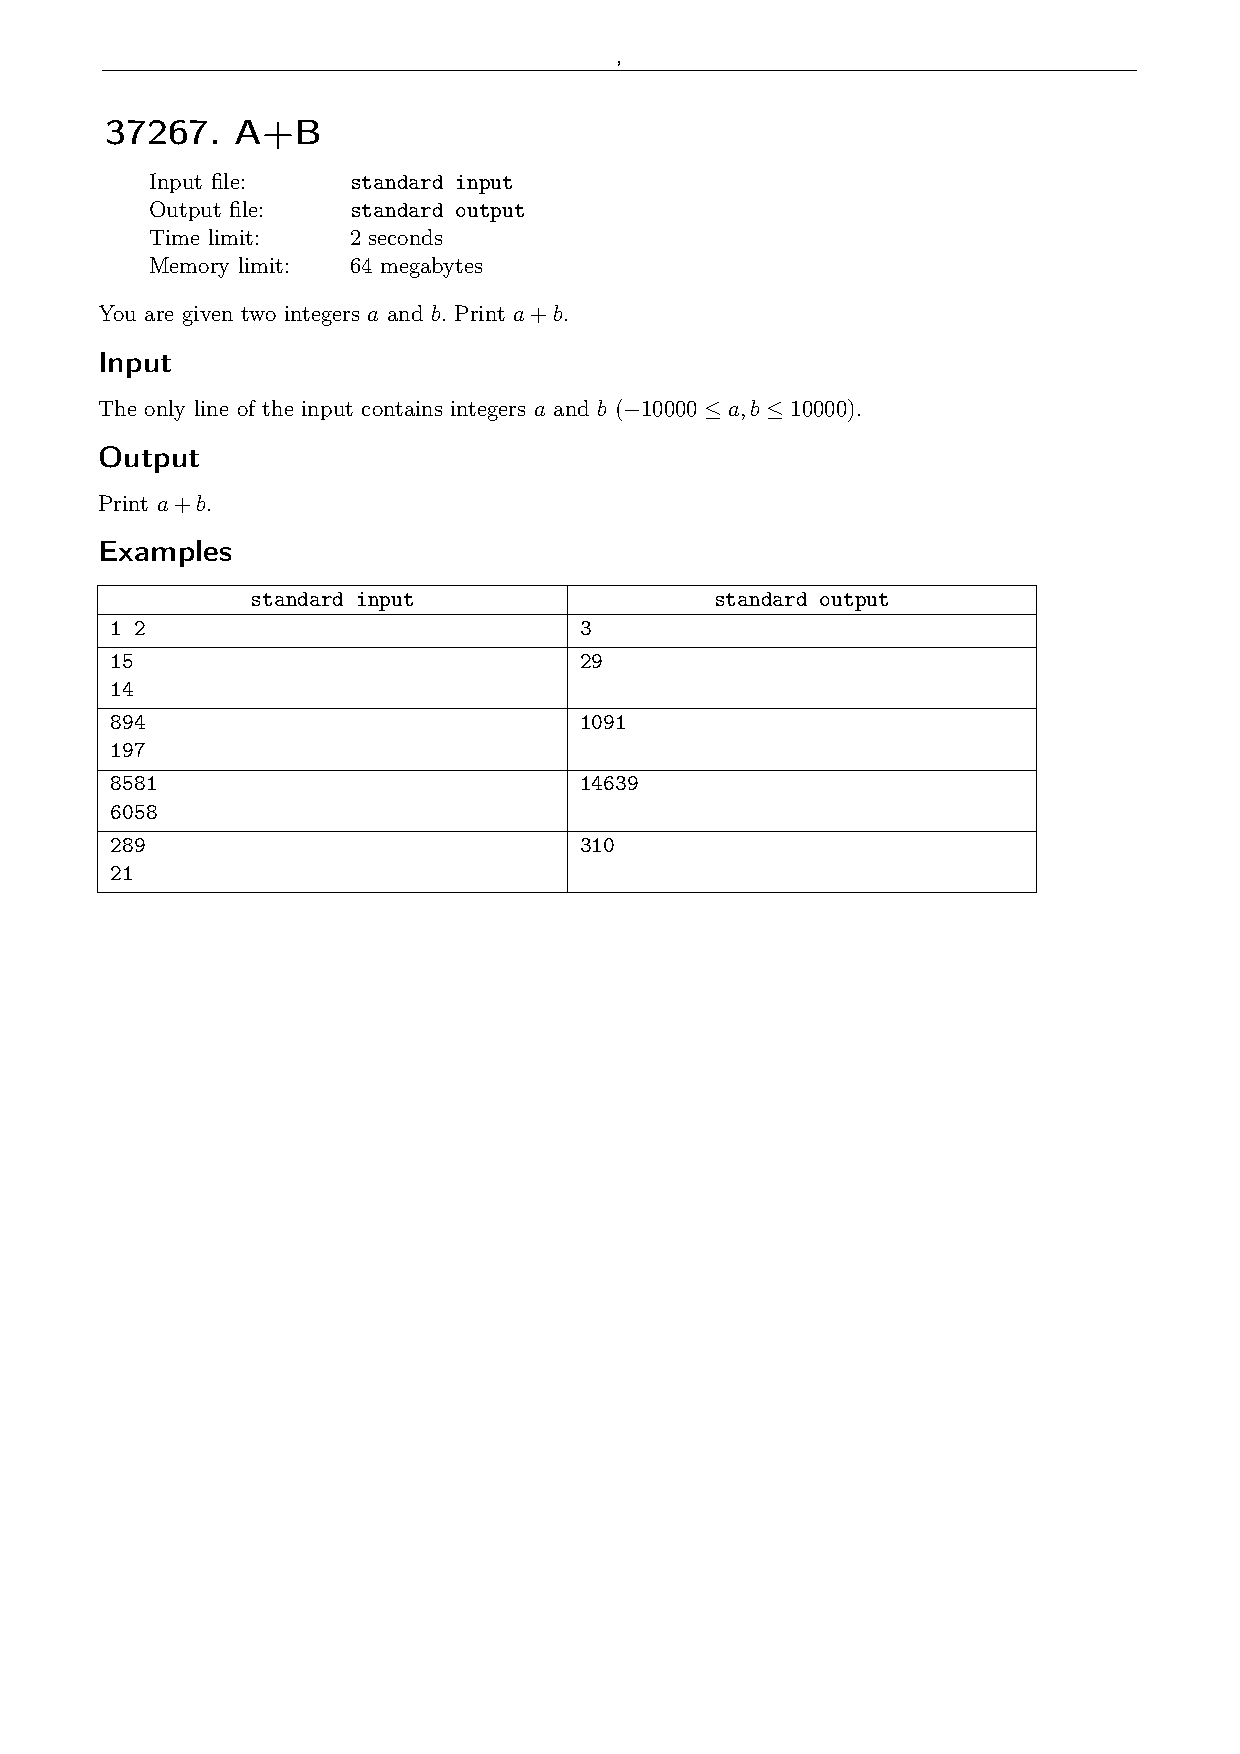
\includepdf[pages=-]{37267.pdf}
    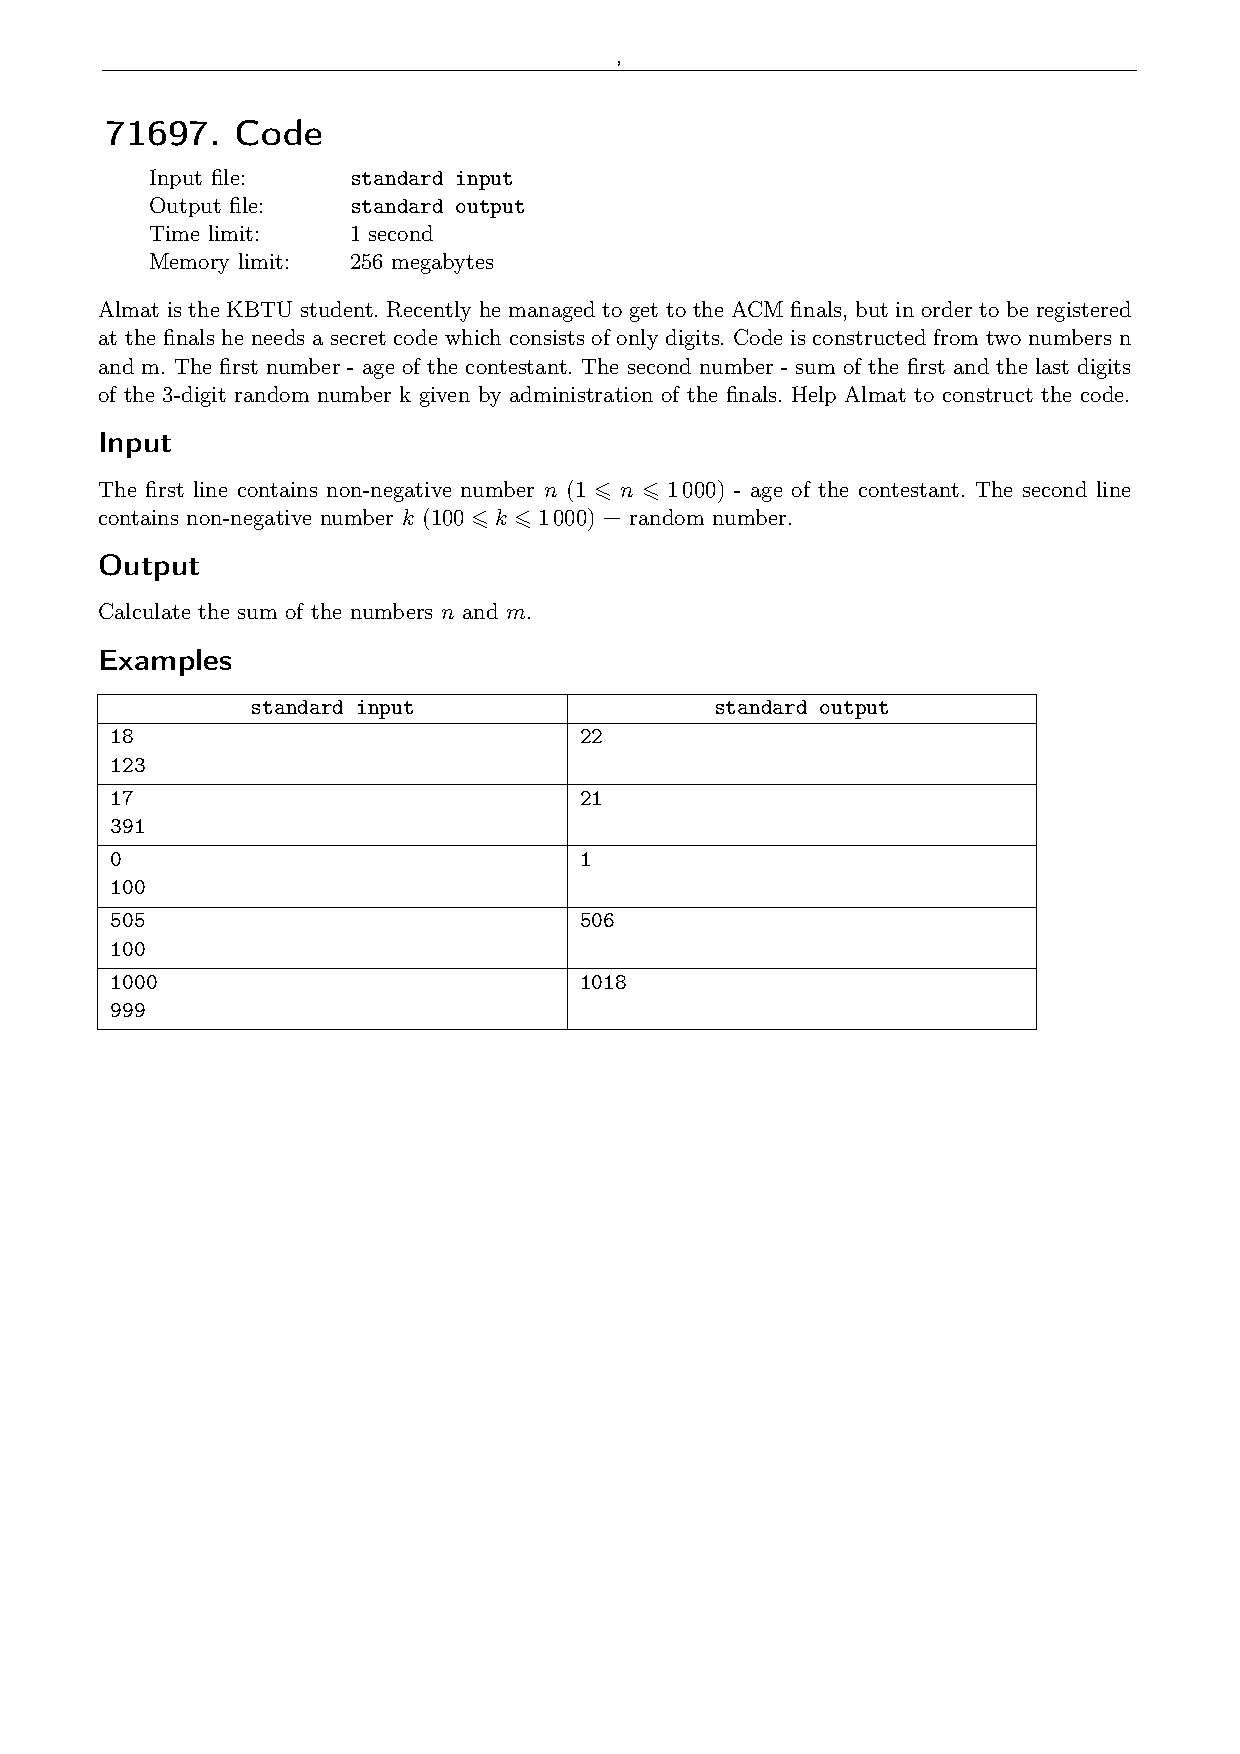
\includepdf[pages=-]{71697.pdf}
    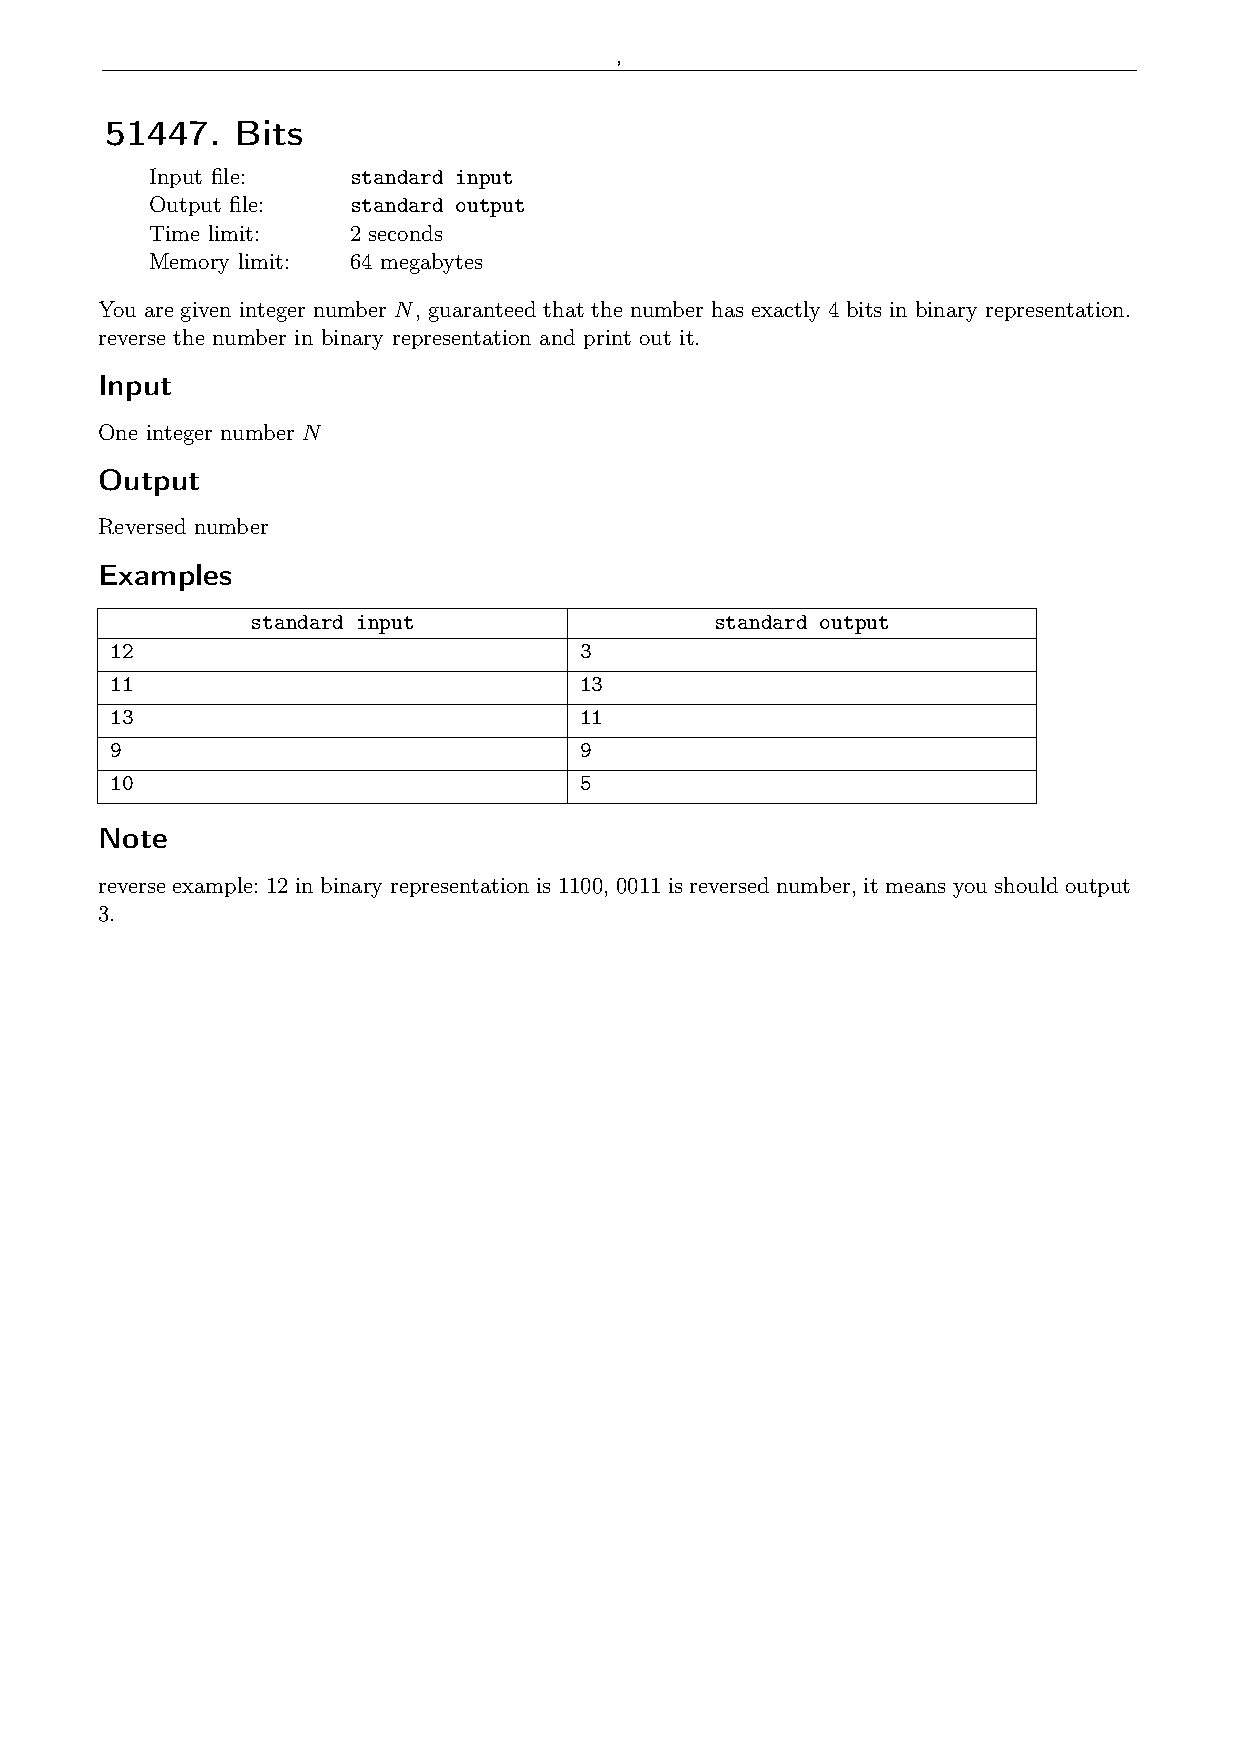
\includepdf[pages=-]{51447.pdf}
    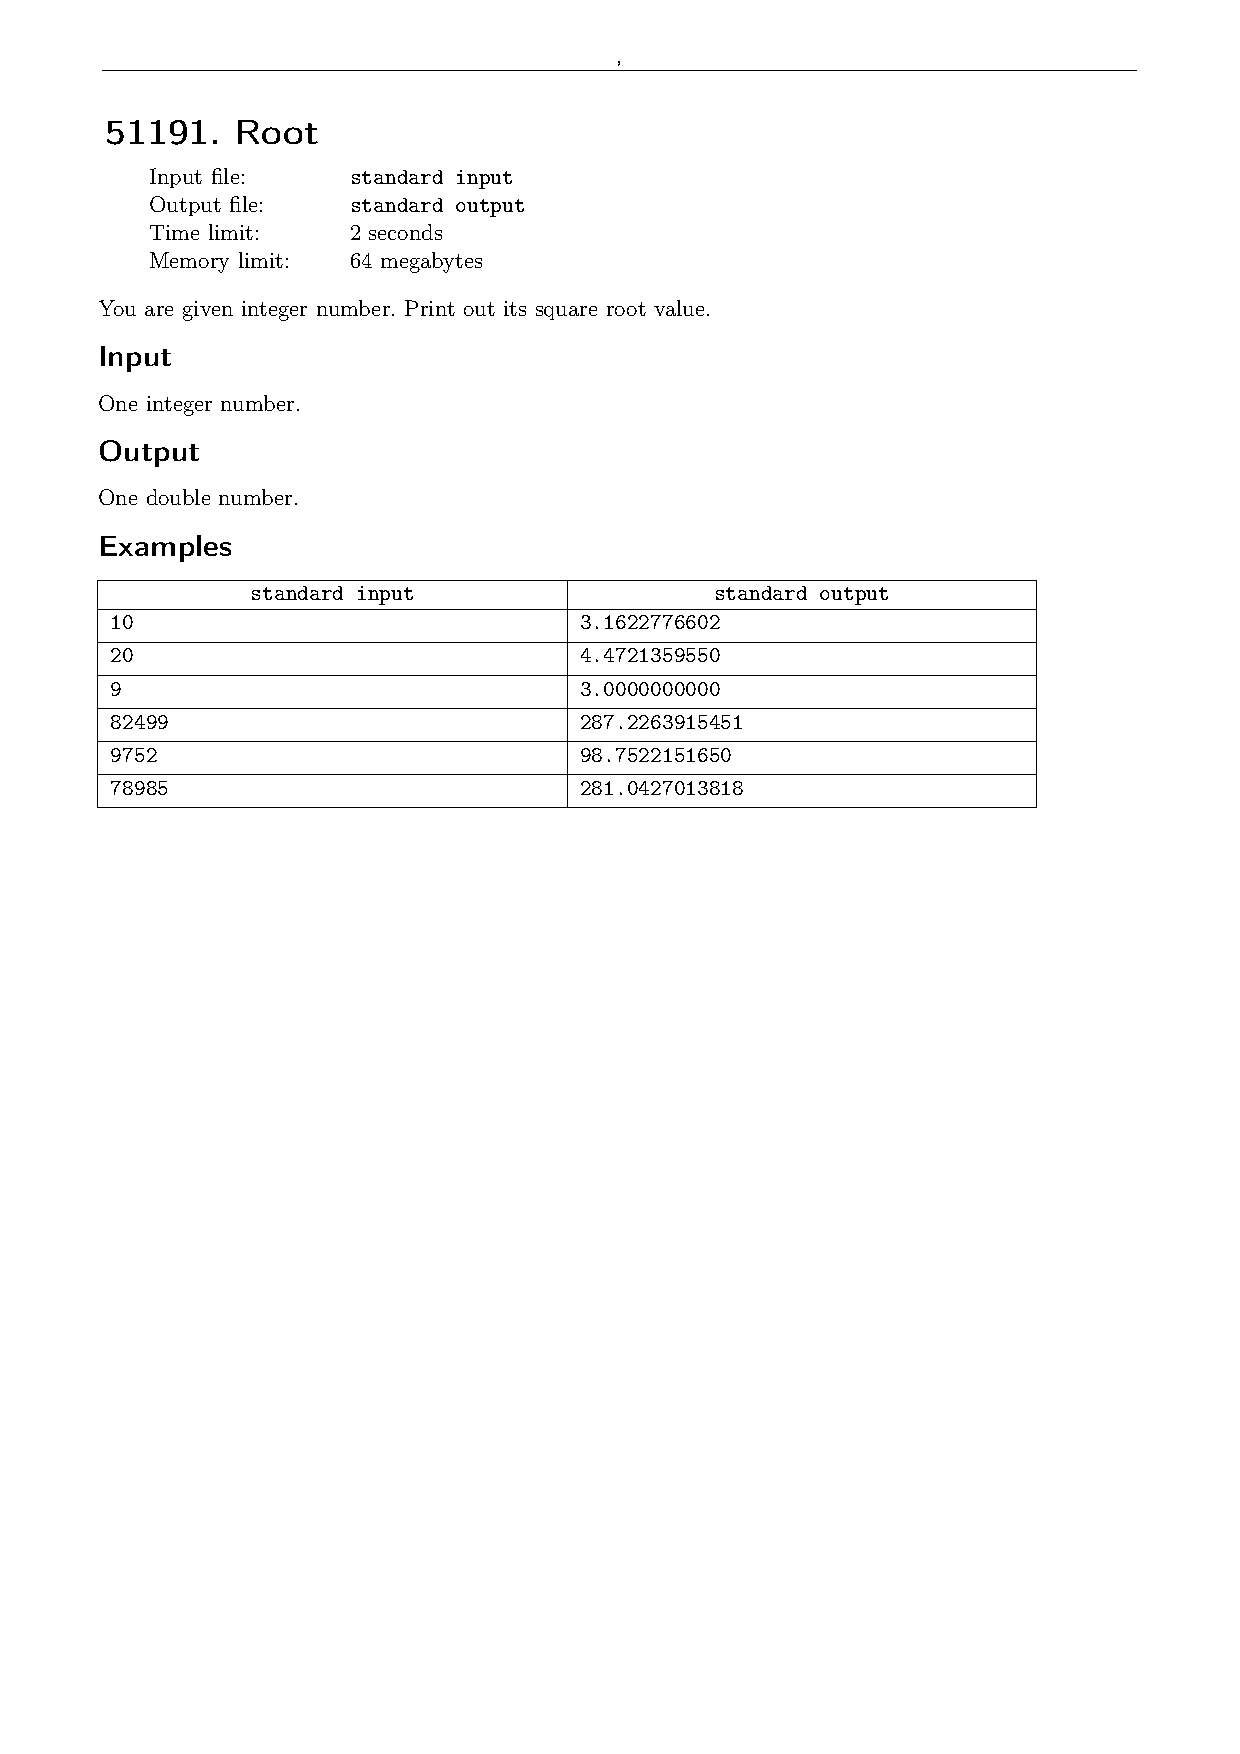
\includepdf[pages=-]{51191.pdf}
    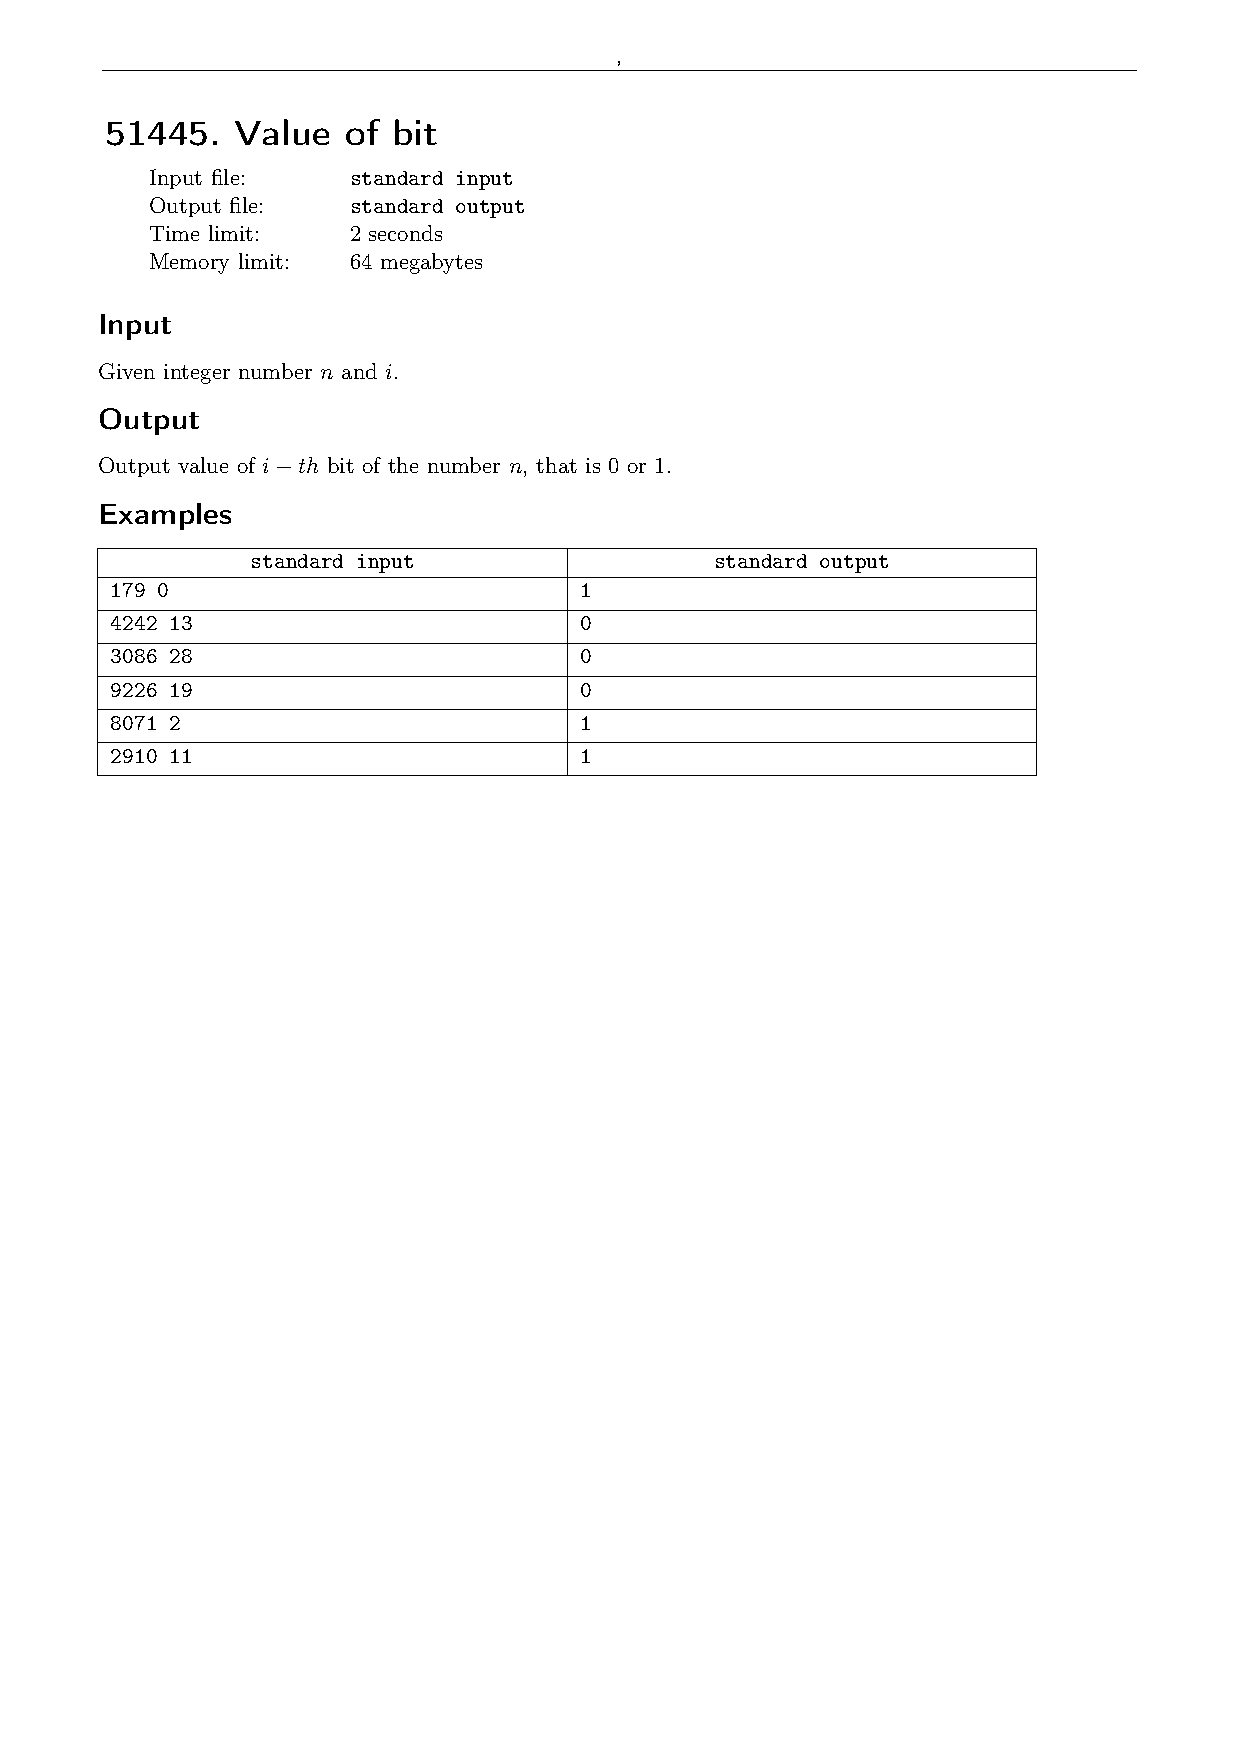
\includepdf[pages=-]{51445.pdf}

    \section{solutions}
    \lstinputlisting{37267.cpp}
    \lstinputlisting{71697.cpp}
    \lstinputlisting{51447.cpp}
    \lstinputlisting{51191.cpp}
    \lstinputlisting{51445.cpp}

    \section{Additional tasks for this lab}
    

\end{document}